% Generated by experiments/make_figures.py.
\definecolor{cA}{HTML}{2a78d6}\definecolor{cB}{HTML}{eb6834}\definecolor{cC}{HTML}{1baf7a}%
\definecolor{cD}{HTML}{4a3aa7}\definecolor{cGray}{HTML}{8a8984}%
\definecolor{lvA}{HTML}{c6dbf5}\definecolor{lvB}{HTML}{93bbec}\definecolor{lvC}{HTML}{5e98e0}%
\definecolor{lvD}{HTML}{2a78d6}\definecolor{lvE}{HTML}{174a8c}\definecolor{lvF}{HTML}{1baf7a}%
\begin{figure}
  \centering
  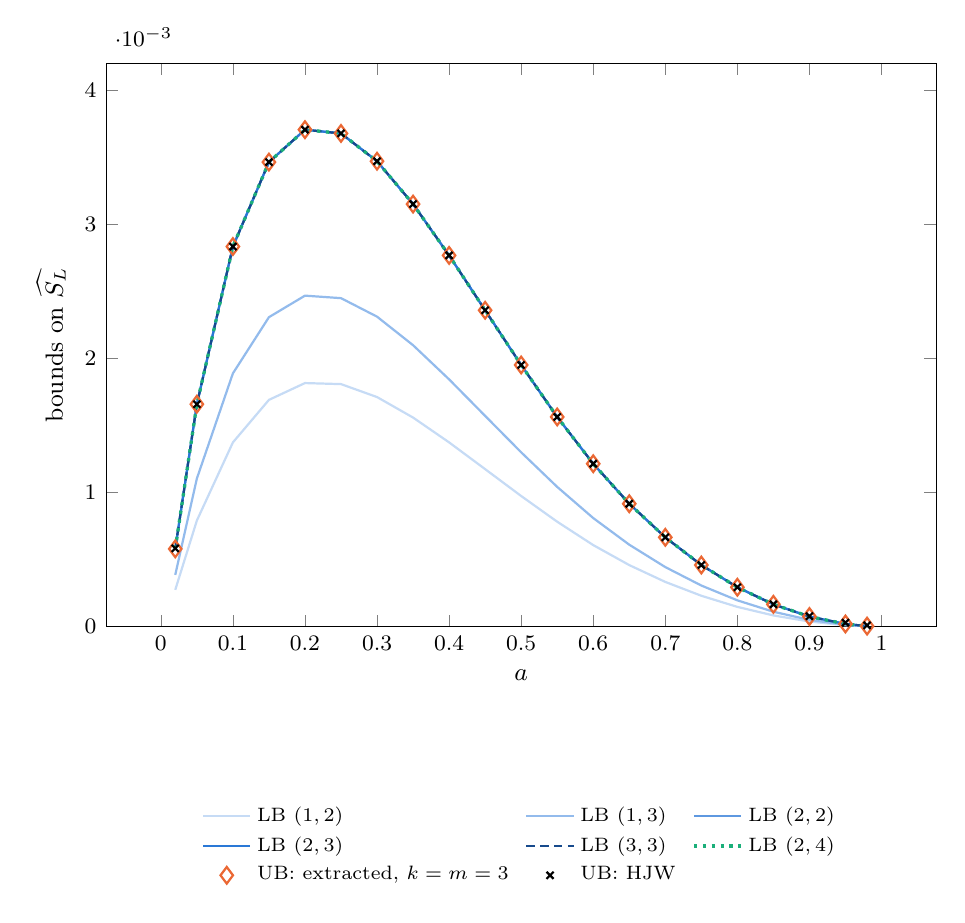
\begin{tikzpicture}
    \begin{axis}[width=\columnwidth, height=0.72\columnwidth, xlabel={$a$}, ylabel={bounds on $\widehat{S_L}$},
      ymin=0, ymax=4.2e-3, scaled y ticks=base 10:3, tick label style={font=\footnotesize}, label style={font=\small},
      legend style={font=\scriptsize, at={(0.5,-0.3)}, anchor=north, draw=none, legend columns=3,
      /tikz/every even column/.append style={column sep=4pt}}, legend cell align=left]
            \addplot[lvA, thick] coordinates {(0.02,0.000273625) (0.05,0.00079074) (0.1,0.0013737) (0.15,0.00169105) (0.2,0.00181649) (0.25,0.00180873) (0.3,0.00171205) (0.35,0.00155909) (0.4,0.00137387) (0.45,0.00117432) (0.5,0.000973725) (0.55,0.000781985) (0.6,0.000607561) (0.65,0.00045823) (0.7,0.000332799) (0.75,0.000229429) (0.8,0.000146488) (0.85,8.26962e-05) (0.9,3.71473e-05) (0.95,9.46255e-06) (0.98,1.53921e-06)};\addlegendentry{LB $(1,2)$}
      \addplot[lvB, thick] coordinates {(0.02,0.000385141) (0.05,0.0011042) (0.1,0.00188876) (0.15,0.00230803) (0.2,0.00246876) (0.25,0.00245005) (0.3,0.00231198) (0.35,0.00209901) (0.4,0.00184413) (0.45,0.00157169) (0.5,0.00129985) (0.55,0.00104174) (0.6,0.000809234) (0.65,0.000610501) (0.7,0.000443453) (0.75,0.000305771) (0.8,0.000195266) (0.85,0.000110238) (0.9,4.95216e-05) (0.95,1.26017e-05) (0.98,2.04489e-06)};\addlegendentry{LB $(1,3)$}
      \addplot[lvC, thick] coordinates {(0.02,0.000578953) (0.05,0.00165879) (0.1,0.00283492) (0.15,0.00346508) (0.2,0.00370697) (0.25,0.00367913) (0.3,0.00347182) (0.35,0.00315192) (0.4,0.00276896) (0.45,0.0023597) (0.5,0.00195135) (0.55,0.00156369) (0.6,0.0012144) (0.65,0.000916041) (0.7,0.000665379) (0.75,0.000458757) (0.8,0.000292954) (0.85,0.000165394) (0.9,7.43038e-05) (0.95,1.89401e-05) (0.98,3.0846e-06)};\addlegendentry{LB $(2,2)$}
      \addplot[lvD, thick] coordinates {(0.02,0.00057896) (0.05,0.00165877) (0.1,0.00283492) (0.15,0.00346508) (0.2,0.00370697) (0.25,0.00367912) (0.3,0.00347182) (0.35,0.00315193) (0.4,0.00276896) (0.45,0.00235969) (0.5,0.00195132) (0.55,0.00156369) (0.6,0.00121439) (0.65,0.00091604) (0.7,0.000665376) (0.75,0.000458755) (0.8,0.000292953) (0.85,0.000165393) (0.9,7.429e-05) (0.95,1.89373e-05) (0.98,3.07865e-06)};\addlegendentry{LB $(2,3)$}
      \addplot[lvE, thick, densely dashed] coordinates {(0.02,0.000578962) (0.05,0.00165879) (0.1,0.00283492) (0.15,0.00346508) (0.2,0.00370698) (0.25,0.00367913) (0.3,0.00347182) (0.35,0.00315192) (0.4,0.00276896) (0.45,0.0023597) (0.5,0.00195136) (0.55,0.00156369) (0.6,0.00121439) (0.65,0.00091604) (0.7,0.000665379) (0.75,0.000458756) (0.8,0.000292954) (0.85,0.000165397) (0.9,7.43057e-05) (0.95,1.8941e-05) (0.98,3.08495e-06)};\addlegendentry{LB $(3,3)$}
      \addplot[lvF, very thick, dotted] coordinates {(0.02,0.000578924) (0.05,0.00165878) (0.1,0.00283491) (0.15,0.00346507) (0.2,0.00370696) (0.25,0.00367909) (0.3,0.0034718) (0.35,0.00315191) (0.4,0.00276894) (0.45,0.00235967) (0.5,0.00195134) (0.55,0.00156366) (0.6,0.00121437) (0.65,0.000916032) (0.7,0.000665365) (0.75,0.000458748) (0.8,0.000292947) (0.85,0.000165389) (0.9,7.42782e-05) (0.95,1.89277e-05) (0.98,3.06766e-06)};\addlegendentry{LB $(2,4)$}
      \addplot[only marks, mark=diamond, mark size=3pt, cB, thick] coordinates {(0.02,0.000579062) (0.05,0.00165889) (0.1,0.00283502) (0.15,0.00346518) (0.2,0.00370708) (0.25,0.00367923) (0.3,0.00347192) (0.35,0.00315202) (0.4,0.00276906) (0.45,0.0023598) (0.5,0.00195146) (0.55,0.00156379) (0.6,0.00121452) (0.65,0.000916171) (0.7,0.000665491) (0.75,0.000458882) (0.8,0.00029305) (0.85,0.000165505) (0.9,7.43634e-05) (0.95,1.89627e-05) (0.98,3.09088e-06)};\addlegendentry{UB: extracted, $k=m=3$}
      \addplot[only marks, mark=x, mark size=2.4pt, black, thick, mark size=1.8pt] coordinates {(0.02,0.000583241) (0.05,0.00165879) (0.1,0.00283492) (0.15,0.00346508) (0.2,0.00370698) (0.25,0.00367913) (0.3,0.00347182) (0.35,0.00315193) (0.4,0.00276896) (0.45,0.0023597) (0.5,0.00195136) (0.55,0.0015637) (0.6,0.0012144) (0.65,0.000916041) (0.7,0.000665379) (0.75,0.000458756) (0.8,0.000292962) (0.85,0.000165633) (0.9,7.7074e-05) (0.95,2.88353e-05) (0.98,8.98313e-06)};\addlegendentry{UB: HJW}
    \end{axis}
  \end{tikzpicture}
  \caption{Convex roof of the linear entropy $S_L=1-\tr\rho_A^2$ for the Horodecki $2\times4$ family
  $\rho_a$. Lines: lower bounds at the levels $(k,m)$ of the simplified hierarchy; from $k=2$ on they coincide, including $(2,4)$ (green, dotted).
  Markers: upper bounds from the decomposition extracted from the SDP solution at $k=m=3$ (orange diamonds) and from
  HJW gradient descent (black crosses).}
  \label{fig:linearEntropy}
\end{figure}
